\documentclass[11pt,a4paper]{report}
\usepackage[textwidth=37em,vmargin=30mm]{geometry}
\usepackage{calc,xunicode,amsmath,amssymb,paralist,enumitem,tabu,booktabs,datetime2,xeCJK,xeCJKfntef,listings}
\usepackage{tocloft,fancyhdr,tcolorbox,xcolor,graphicx,eso-pic,xltxtra,xelatexemoji}

\newcommand{\envyear}[0]{2025}
\newcommand{\envdatestr}[0]{2025-02-28}
\newcommand{\envfinaldir}[0]{webdb/2025/20250228/final}

\usepackage[hidelinks]{hyperref}
\hypersetup{
    colorlinks=false,
    pdfpagemode=FullScreen,
    pdftitle={Web Digest - \envdatestr}
}

\setlength{\cftbeforechapskip}{10pt}
\renewcommand{\cftchapfont}{\rmfamily\bfseries\large\raggedright}
\setlength{\cftbeforesecskip}{2pt}
\renewcommand{\cftsecfont}{\sffamily\small\raggedright}

\setdefaultleftmargin{2em}{2em}{1em}{1em}{1em}{1em}

\usepackage{xeCJK,xeCJKfntef}
\xeCJKsetup{PunctStyle=plain,RubberPunctSkip=false,CJKglue=\strut\hskip 0pt plus 0.1em minus 0.05em,CJKecglue=\strut\hskip 0.22em plus 0.2em}
\XeTeXlinebreaklocale "zh"
\XeTeXlinebreakskip = 0pt


\setmainfont{Brygada 1918}
\setromanfont{Brygada 1918}
\setsansfont{IBM Plex Sans}
\setmonofont{JetBrains Mono NL}
\setCJKmainfont{Noto Serif CJK SC}
\setCJKromanfont{Noto Serif CJK SC}
\setCJKsansfont{Noto Sans CJK SC}
\setCJKmonofont{Noto Sans CJK SC}

\setlength{\parindent}{0pt}
\setlength{\parskip}{8pt}
\linespread{1.15}

\lstset{
	basicstyle=\ttfamily\footnotesize,
	numbersep=5pt,
	backgroundcolor=\color{black!5},
	showspaces=false,
	showstringspaces=false,
	showtabs=false,
	tabsize=2,
	captionpos=b,
	breaklines=true,
	breakatwhitespace=true,
	breakautoindent=true,
	linewidth=\textwidth
}






\newcommand{\coverpic}[2]{
    % argv: itemurl, authorname
    Cover photo by #2~~(\href{#1}{#1})
}
\newcommand{\makeheader}[0]{
    \begin{titlepage}
        % \newgeometry{hmargin=15mm,tmargin=21mm,bmargin=12mm}
        \begin{center}
            
            \rmfamily\scshape
            \fontspec{BaskervilleF}
            \fontspec{Old Standard}
            \fontsize{59pt}{70pt}\selectfont
            WEB\hfill DIGEST
            
            \vfill
            % \vskip 30pt
            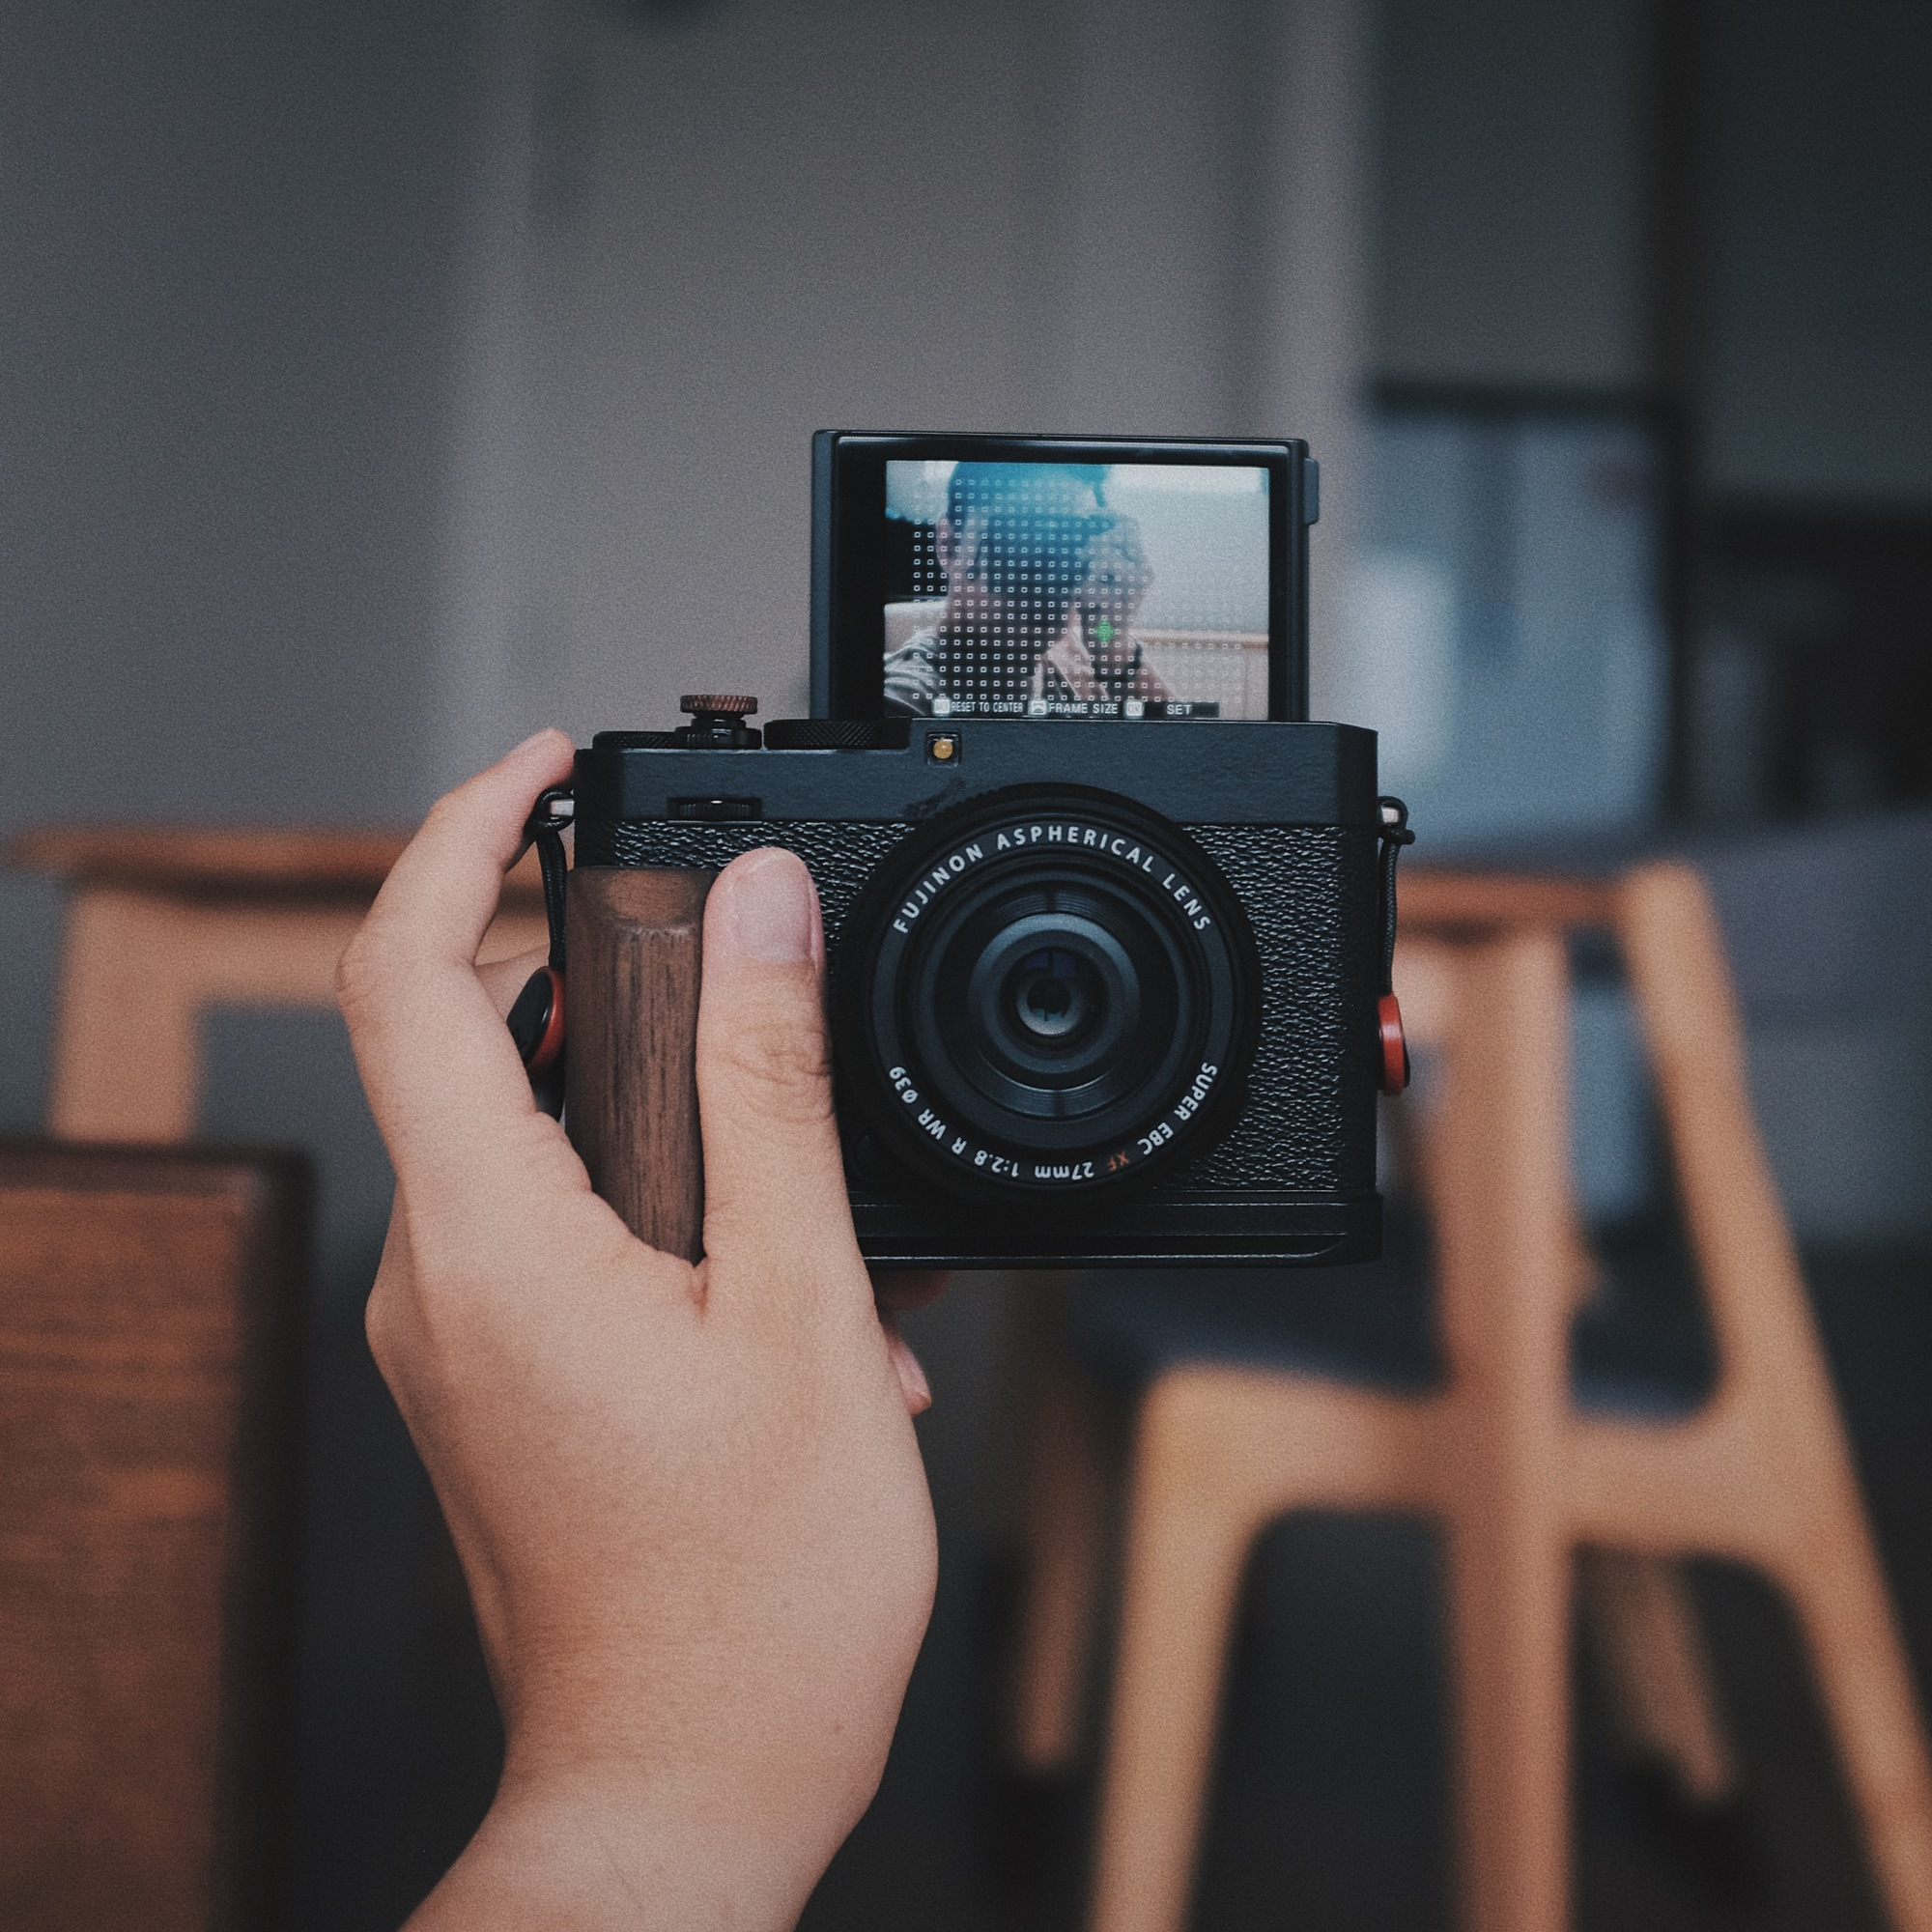
\includegraphics[width=\linewidth]{\envfinaldir/coverpic-prod.jpg}\par
            % \vskip 30pt
            \vfill

            \normalsize\rmfamily\scshape
            \copyright{} The Web Digest Project \hfill\large \envdatestr
        \end{center}
    \end{titlepage}
    % \restoregeometry
}
\newcommand{\simplehref}[1]{%
    \textcolor{blue!80!green}{\href{#1}{#1}}%
}
\renewcommand{\contentsname}{\center\Huge\sffamily\bfseries Contents\par\vskip 20pt}
\newcounter{ipartcounter}
\setcounter{ipartcounter}{0}
\newcommand{\ipart}[1]{
    % \vskip 20pt
    \clearpage
    \stepcounter{ipartcounter}
    \phantomsection
    \addcontentsline{toc}{chapter}{#1}
    % \begin{center}
    %     \Huge
    %     \sffamily\bfseries
    %     #1
    % \end{center}
    % \vskip 20pt plus 7pt
}
\newcounter{ichaptercounter}
\setcounter{ichaptercounter}{0}
\newcommand{\ichapter}[1]{
    % \vskip 20pt
    \clearpage
    \stepcounter{ichaptercounter}
    \phantomsection
    \addcontentsline{toc}{section}{\numberline{\arabic{ichaptercounter}}#1}
    \begin{center}
        \Huge
        \sffamily\bfseries
        #1
    \end{center}
    \vskip 20pt plus 7pt
}
\newcommand{\entrytitlefont}[1]{\subsection*{\raggedright\Large\sffamily\bfseries#1}}
\newcommand{\entryitemGeneric}[2]{
    % argv: title, url
    \parbox{\linewidth}{
        \entrytitlefont{#1}\par\vskip 5pt
        \footnotesize\ttfamily\mdseries
        \simplehref{#2}
    }\vskip 11pt plus 11pt minus 1pt
}
\newcommand{\entryitemGithub}[3]{
    % argv: title, url, desc
    \parbox{\linewidth}{
        \entrytitlefont{#1}\par\vskip 5pt
        \footnotesize\ttfamily\mdseries
        \simplehref{#2}\par\vskip 5pt
        \small\rmfamily\mdseries#3
    }\vskip 11pt plus 11pt minus 1pt
}
\newcommand{\entryitemAp}[3]{
    % argv: title, url, desc
    \parbox{\linewidth}{
        \entrytitlefont{#1}\par\vskip 5pt
        \footnotesize\ttfamily\mdseries
        \simplehref{#2}\par\vskip 5pt
        \small\rmfamily\mdseries#3
    }\vskip 11pt plus 11pt minus 1pt
}
\newcommand{\entryitemHackernews}[3]{
    % argv: title, hnurl, rawurl
    % \parbox{\linewidth}{
    %     \entrytitlefont{#1}\par\vskip 5pt
    %     \footnotesize\ttfamily\mdseries
    %     \simplehref{#3}\par
    %     \textcolor{black!50}{\href{#2}{#2}}
    % }\vskip 11pt plus 11pt minus 1pt
    \begin{minipage}{\linewidth}
            \entrytitlefont{#1}\par\vskip 5pt
            \footnotesize\ttfamily\mdseries
            \simplehref{#3}\par
            \textcolor{black!50}{\href{#2}{#2}}
    \end{minipage}\par\vskip 11pt plus 11pt minus 1pt
}







\begin{document}

\makeheader

\tableofcontents\clearpage




\ipart{Developers}
\ichapter{Hacker News}
\entryitemTwoLinks{Carlos Slim cancels his collaboration with Elon Musk's Starlink}{https://news.ycombinator.com/item?id=43199362}{https://mexicodailypost.com/2025/02/24/carlos-slim-orders-to-cancel-his-collaboration-with-elon-musks-starlink/}

\entryitemTwoLinks{IBM Completes Acquisition of HashiCorp}{https://news.ycombinator.com/item?id=43199256}{https://newsroom.ibm.com/2025-02-27-ibm-completes-acquisition-of-hashicorp,-creates-comprehensive,-end-to-end-hybrid-cloud-platform}

\entryitemTwoLinks{GPT-4.5}{https://news.ycombinator.com/item?id=43197872}{https://openai.com/index/introducing-gpt-4-5/}

\entryitemTwoLinks{EA Open Sources Command and Conquer: Red Alert}{https://news.ycombinator.com/item?id=43197131}{https://github.com/electronicarts/CnC\_Red\_Alert}

\entryitemTwoLinks{Goodbye K-9 Mail}{https://news.ycombinator.com/item?id=43196436}{https://cketti.de/2025/02/26/goodbye-k9mail/}

\entryitemTwoLinks{Show HN: Superglue – open source API connector that writes its own code}{https://news.ycombinator.com/item?id=43196374}{https://github.com/superglue-ai/superglue}

\entryitemTwoLinks{Turning a Bluetooth device into an Apple AirTag without root privileges}{https://news.ycombinator.com/item?id=43196207}{https://nroottag.github.io/}

\entryitemTwoLinks{Distributed systems programming has stalled}{https://news.ycombinator.com/item?id=43195702}{https://www.shadaj.me/writing/distributed-programming-stalled}

\entryitemTwoLinks{A \$100 DIY muon tomographer}{https://news.ycombinator.com/item?id=43195525}{https://spectrum.ieee.org/diy-muon-tomography}

\entryitemTwoLinks{Solitaire}{https://news.ycombinator.com/item?id=43195516}{https://localthunk.com/blog/solitaire}

\entryitemTwoLinks{Show HN: Probly – Spreadsheets, Python, and AI in the browser}{https://news.ycombinator.com/item?id=43194971}{https://github.com/PragmaticMachineLearning/probly}

\entryitemTwoLinks{Mozilla's new terms of use are out of step with Firefox's direct competition}{https://news.ycombinator.com/item?id=43194536}{https://www.quippd.com/writing/2025/02/26/mozillas-new-terms-of-use-are-out-of-step-with-firefoxs-direct-competition.html}

\entryitemTwoLinks{Fish 4}{https://news.ycombinator.com/item?id=43194024}{https://github.com/fish-shell/fish-shell/releases/tag/4.0.0}

\entryitemTwoLinks{A data analysis of speeches at the Oscars}{https://news.ycombinator.com/item?id=43193714}{https://stephenfollows.com/p/harvey-weinstein-thanked-more-than-god}

\entryitemTwoLinks{US Forest Service firings decimate already understaffed agency}{https://news.ycombinator.com/item?id=43193366}{https://grist.org/politics/forest-service-firings-decimate-already-understaffed-agency/}

\entryitemTwoLinks{RoboPianist: Dexterous Piano Playing with Deep Reinforcement Learning (2023)}{https://news.ycombinator.com/item?id=43192751}{https://kzakka.com/robopianist/\#demo}

\entryitemTwoLinks{Gene Hackman has died}{https://news.ycombinator.com/item?id=43192500}{https://www.nytimes.com/2025/02/27/obituaries/gene-hackman-dead.html}

\entryitemTwoLinks{Teslas monitor everything – including you [video] from WIRED}{https://news.ycombinator.com/item?id=43192079}{https://www.youtube.com/watch?v=l7VHsDODU7E}

\entryitemTwoLinks{DualPipe: Bidirectional pipeline parallelism algorithm}{https://news.ycombinator.com/item?id=43190533}{https://github.com/deepseek-ai/DualPipe}

\entryitemTwoLinks{DeepSeek Open Source Optimized Parallelism Strategies, 3 repos}{https://news.ycombinator.com/item?id=43190482}{https://github.com/deepseek-ai/profile-data}\ichapter{Phoronix}
\entryitemGeneric{\hskip 0pt{}Intel Posts Linux Kernel Patches For Supporting APX - Advanced Performance Extensions}{https://www.phoronix.com/news/Intel-APX-Linux-Kernel-Patches}

\entryitemGeneric{\hskip 0pt{}EA Open-Sources Command \& Conquer Red Alert}{https://www.phoronix.com/news/EA-Open-Source-CnC-Red-Alert}

\entryitemGeneric{\hskip 0pt{}Motion Control Subsystem Proposed For The Linux Kernel}{https://www.phoronix.com/news/Linux-Motion-Control-Subsystem}

\entryitemGeneric{\hskip 0pt{}SUSE's "Agama" OS Installer Receives Pleasant Facelift, Future Roadmap}{https://www.phoronix.com/news/SUSE-Agama-12-Released}

\entryitemGeneric{\hskip 0pt{}NVIDIA 570.124.04 Linux Driver Brings Additional Fixes}{https://www.phoronix.com/news/NVIDIA-570.124.04-Linux-Driver}

\entryitemGeneric{\hskip 0pt{}FFmpeg Lands AV1 RTP Packetizer/Depacketizer}{https://www.phoronix.com/news/FFmpeg-AV1-RTP-Packetizer}

\entryitemGeneric{\hskip 0pt{}FreeBSD In Q4 Saw More Work For AMD Systems, Framework Laptops \& PinePhone Pro}{https://www.phoronix.com/news/FreeBSD-Q4-2024}

\entryitemGeneric{\hskip 0pt{}Fish 4.0 Shell Released With Code Ported From C++ To Rust}{https://www.phoronix.com/news/Fish-Shell-4.0-Released}

\entryitemGeneric{\hskip 0pt{}AMD Open-Sources GMLIB For RadeonSI Driver - Working On HDR Video Support}{https://www.phoronix.com/news/AMD-GMLIB-RadeonSI-HDR-Video}\ichapter{Dribbble}
\entryitemGeneric{\hskip 0pt{}Letter A}{https://dribbble.com/shots/25691267-Letter-A}

\entryitemGeneric{\hskip 0pt{}Tally Logo Design}{https://dribbble.com/shots/25693309-Tally-Logo-Design}

\entryitemGeneric{\hskip 0pt{}Ramotion Logo Design}{https://dribbble.com/shots/25582478-Ramotion-Logo-Design}

\entryitemGeneric{\hskip 0pt{}Cimet Stationery}{https://dribbble.com/shots/25687823-Cimet-Stationery}

\entryitemGeneric{\hskip 0pt{}Letter a}{https://dribbble.com/shots/25680095-Letter-a}

\entryitemGeneric{\hskip 0pt{}auren - logo design}{https://dribbble.com/shots/25681046-auren-logo-design}

\entryitemGeneric{\hskip 0pt{}Block13 Skateboards \& Sreetwear}{https://dribbble.com/shots/25683504-Block13-Skateboards-Sreetwear}

\entryitemGeneric{\hskip 0pt{}Quokka Mascot}{https://dribbble.com/shots/25681470-Quokka-Mascot}

\entryitemGeneric{\hskip 0pt{}Cardi C}{https://dribbble.com/shots/25678066-Cardi-C}

\entryitemGeneric{\hskip 0pt{}R}{https://dribbble.com/shots/25673587-R}

\entryitemGeneric{\hskip 0pt{}Fitme home landing page}{https://dribbble.com/shots/25674639-Fitme-home-landing-page}

\entryitemGeneric{\hskip 0pt{}Illustrated Icons - American Home Shield}{https://dribbble.com/shots/25666386-Illustrated-Icons-American-Home-Shield}

\entryitemGeneric{\hskip 0pt{}Triceratops Dino}{https://dribbble.com/shots/25676249-Triceratops-Dino}

\entryitemGeneric{\hskip 0pt{}Unused Geometric Fox}{https://dribbble.com/shots/25677006-Unused-Geometric-Fox}

\entryitemGeneric{\hskip 0pt{}Tiger Style}{https://dribbble.com/shots/25676567-Tiger-Style}

\entryitemGeneric{\hskip 0pt{}Logo Tip 002. Rhythm in Logo Design}{https://dribbble.com/shots/25674872-Logo-Tip-002-Rhythm-in-Logo-Design}

\entryitemGeneric{\hskip 0pt{}The Business}{https://dribbble.com/shots/25676385-The-Business}

\entryitemGeneric{\hskip 0pt{}Cute Dinosaur}{https://dribbble.com/shots/25671549-Cute-Dinosaur}

\entryitemGeneric{\hskip 0pt{}BNPL service}{https://dribbble.com/shots/25664920-BNPL-service}

\entryitemGeneric{\hskip 0pt{}Wolf Creek Golf Club}{https://dribbble.com/shots/25664483-Wolf-Creek-Golf-Club}

\entryitemGeneric{\hskip 0pt{}Business illustration set}{https://dribbble.com/shots/25661493-Business-illustration-set}

\entryitemGeneric{\hskip 0pt{}b}{https://dribbble.com/shots/25663031-b}

\entryitemGeneric{\hskip 0pt{}ProAWS Logo Design}{https://dribbble.com/shots/25661915-ProAWS-Logo-Design}

\entryitemGeneric{\hskip 0pt{}—From Archive (Pt. 8)}{https://dribbble.com/shots/25663911--From-Archive-Pt-8}


\ipart{Developers~~~~(zh-Hans)}
\ichapter{Solidot}
\entryitemGeneric{\hskip 0pt{}Fish Shell 4.0 释出}{https://www.solidot.org/story?sid=80672}

\entryitemGeneric{\hskip 0pt{}激素疗法或有助于延缓皮肤衰老}{https://www.solidot.org/story?sid=80671}

\entryitemGeneric{\hskip 0pt{}Ocean Infinity 重新开始搜寻 MH370}{https://www.solidot.org/story?sid=80670}

\entryitemGeneric{\hskip 0pt{}暗能量光谱仪发现 2800 个候选黑洞}{https://www.solidot.org/story?sid=80669}

\entryitemGeneric{\hskip 0pt{}东京推行四天工作制试图平衡工作和生活}{https://www.solidot.org/story?sid=80668}

\entryitemGeneric{\hskip 0pt{}Firefox 公布使用条款和更新隐私条款}{https://www.solidot.org/story?sid=80667}

\entryitemGeneric{\hskip 0pt{}Automattic 可能面临集体诉讼}{https://www.solidot.org/story?sid=80666}

\entryitemGeneric{\hskip 0pt{}中国湿地总面积过去四十年净减少 6 万平方公里}{https://www.solidot.org/story?sid=80665}

\entryitemGeneric{\hskip 0pt{}极端高温可能进一步加速老年人衰老}{https://www.solidot.org/story?sid=80664}

\entryitemGeneric{\hskip 0pt{}新发现再次否定了佩托悖论}{https://www.solidot.org/story?sid=80663}

\entryitemGeneric{\hskip 0pt{}《半条命 3》可能进入到了开发的最后阶段}{https://www.solidot.org/story?sid=80662}

\entryitemGeneric{\hskip 0pt{}一种新骨髓移植法能治愈镰状细胞贫血症}{https://www.solidot.org/story?sid=80661}

\entryitemGeneric{\hskip 0pt{}内燃机汽车销量已达峰值开始下降}{https://www.solidot.org/story?sid=80660}

\entryitemGeneric{\hskip 0pt{}小行星 2024 YR4 撞击地球概率下调至 0.004\%}{https://www.solidot.org/story?sid=80659}

\entryitemGeneric{\hskip 0pt{}Y 孵化器支持的 AI 公司被批评其产品是在虐待工厂工人}{https://www.solidot.org/story?sid=80658}

\entryitemGeneric{\hskip 0pt{}前工业化社群睡眠时间更短}{https://www.solidot.org/story?sid=80657}

\entryitemGeneric{\hskip 0pt{}高通和 Google 合作为 Android 提供最高八年的更新}{https://www.solidot.org/story?sid=80656}

\entryitemGeneric{\hskip 0pt{}皮尤调查发现大部分美国工人避用 AI 聊天机器人}{https://www.solidot.org/story?sid=80655}

\entryitemGeneric{\hskip 0pt{}Mozilla 重申会继续支持 Manifest v2 扩展}{https://www.solidot.org/story?sid=80654}

\entryitemGeneric{\hskip 0pt{}Framework 推出三款新产品,包括 128GB 内存 Ryzen AI Max+ 395 小主机}{https://www.solidot.org/story?sid=80653}\ichapter{V2EX}
\entryitemGeneric{\hskip 0pt{}[优惠信息] 京东自营的 mac 已经支持教育优惠+国补了}{https://www.v2ex.com/t/1114768}

\entryitemGeneric{\hskip 0pt{}[求职] [求职][技术交流]求一份 DTS(Data Transfer Service)方向的工作}{https://www.v2ex.com/t/1114767}

\entryitemGeneric{\hskip 0pt{}[汽车] 老生常谈的话题了,今早上海大雾。}{https://www.v2ex.com/t/1114766}

\entryitemGeneric{\hskip 0pt{}[分享发现] 发现一个新的 JVM 构建工具 Mill}{https://www.v2ex.com/t/1114764}

\entryitemGeneric{\hskip 0pt{}[Steam] 《命令与征服:将军》和资料片《绝命时刻》的源代码已经以 GPL 3.0 协议开放}{https://www.v2ex.com/t/1114763}

\entryitemGeneric{\hskip 0pt{}[问与答] 电脑清灰,是选择涵道风机还是压缩空气?}{https://www.v2ex.com/t/1114762}

\entryitemGeneric{\hskip 0pt{}[Apple] JD 可以买 2999 的 Mac Mini 了,实测北京可以}{https://www.v2ex.com/t/1114761}

\entryitemGeneric{\hskip 0pt{}[VXNA] 申请收录个人博客: 极北人工智障}{https://www.v2ex.com/t/1114760}

\entryitemGeneric{\hskip 0pt{}[程序员] 实验室 GPU 集群管理经验分享与问题探讨,求建议}{https://www.v2ex.com/t/1114759}

\entryitemGeneric{\hskip 0pt{}[云计算] 移动云网络怎么样}{https://www.v2ex.com/t/1114758}

\entryitemGeneric{\hskip 0pt{}[全球工单系统] 腾讯会议 64 位安装包是不是坏了}{https://www.v2ex.com/t/1114756}

\entryitemGeneric{\hskip 0pt{}[程序员] AI 在编程领域可能会革掉 Java / Python 的命?}{https://www.v2ex.com/t/1114755}

\entryitemGeneric{\hskip 0pt{}[OpenAI] 看样子 OpenAI 要发布 GPT-4.5 了 AI 圈要轮流争第一}{https://www.v2ex.com/t/1114754}

\entryitemGeneric{\hskip 0pt{}[Tesla] 我看现在网上 fsd 被吐槽,有没有做智能驾驶的专业人士来评价看看,现在 fsd 的水平,以及未来会不会成为公认的 top0}{https://www.v2ex.com/t/1114753}

\entryitemGeneric{\hskip 0pt{}[哔哩哔哩] B 站绑定邮箱的操蛋之处。。。}{https://www.v2ex.com/t/1114752}

\entryitemGeneric{\hskip 0pt{}[程序员] 想请教一个问题, cloudflare worker 怎么限制只有自己另外的的 worker 可以访问呢?}{https://www.v2ex.com/t/1114751}

\entryitemGeneric{\hskip 0pt{}[OpenAI] 字节的 trae,上线 Claude 3.7,实测可用}{https://www.v2ex.com/t/1114749}

\entryitemGeneric{\hskip 0pt{}[问与答] ComfyUI 模型,在 Citiviai 上面下了 lora,各种参数均一样,跑出来效果却不一样}{https://www.v2ex.com/t/1114748}

\entryitemGeneric{\hskip 0pt{}[问与答] 有老哥订阅了这个么 有偿求一个}{https://www.v2ex.com/t/1114747}

\entryitemGeneric{\hskip 0pt{}[问与答] 500 以内码代码用键盘,求推荐}{https://www.v2ex.com/t/1114746}

\entryitemGeneric{\hskip 0pt{}[深圳] 朋友们,新手司机,请问南山哪里停车性价比高}{https://www.v2ex.com/t/1114745}

\entryitemGeneric{\hskip 0pt{}[程序员] 为什么 Android、iOS 上没有 Electron 这样能一键把网站变成用起来接近 Native 体验的框架?我以前也是天天黑电子垃圾,相当于往电脑上装了十几个 Chrome 、ffmpeg 。但是 Electron 这几年进步确实猛}{https://www.v2ex.com/t/1114744}

\entryitemGeneric{\hskip 0pt{}[Apple] 巨魔不了的情况下,有必要买个证书吗?}{https://www.v2ex.com/t/1114743}

\entryitemGeneric{\hskip 0pt{}[OpenAI] closeai 除了封号,现在又开始共享号检测了。}{https://www.v2ex.com/t/1114742}

\entryitemGeneric{\hskip 0pt{}[职场话题] 极氪上海徐汇外包能不能去?}{https://www.v2ex.com/t/1114741}

\entryitemGeneric{\hskip 0pt{}[Apple] IOS 的推送通知问题}{https://www.v2ex.com/t/1114740}

\entryitemGeneric{\hskip 0pt{}[商业模式] 从副业发展出来的一个人公司,靠这种模式年入 130 万美元!}{https://www.v2ex.com/t/1114739}

\entryitemGeneric{\hskip 0pt{}[问与答] 2000 块钱以下,有没有好用的 windows 笔记本推荐,便于携带,日常工作需要}{https://www.v2ex.com/t/1114738}

\entryitemGeneric{\hskip 0pt{}[分享发现] 分享移民加拿大的时间线}{https://www.v2ex.com/t/1114737}

\entryitemGeneric{\hskip 0pt{}[职场话题] 干了六年的同事自己辞职了,桌上留下了六张生日卡。}{https://www.v2ex.com/t/1114736}

\entryitemGeneric{\hskip 0pt{}[投资] 小米股票收益}{https://www.v2ex.com/t/1114735}

\entryitemGeneric{\hskip 0pt{}[健康] 今日去医院看病有感}{https://www.v2ex.com/t/1114734}

\entryitemGeneric{\hskip 0pt{}[汽车] su7 ultra 才 52.99 万,兄弟们买吗?一年工资就够了吧!}{https://www.v2ex.com/t/1114733}

\entryitemGeneric{\hskip 0pt{}[分享创造] 随 AI 大流,用 AI 建了个站,用来临时分享联系方式,站名:联盾}{https://www.v2ex.com/t/1114732}

\entryitemGeneric{\hskip 0pt{}[问与答] 失业,要不要回老家呢}{https://www.v2ex.com/t/1114731}

\entryitemGeneric{\hskip 0pt{}[分享创造] Kee 2.0 发布,更简单、更美观的创建你的在线 home screen}{https://www.v2ex.com/t/1114730}

\entryitemGeneric{\hskip 0pt{}[酷工作] [上海]得物-交易平台- Java 开发工程师/专家(薪资面议)}{https://www.v2ex.com/t/1114729}

\entryitemGeneric{\hskip 0pt{}[宽带症候群] 河北联通又大规模限制 5Mbps 了}{https://www.v2ex.com/t/1114728}

\entryitemGeneric{\hskip 0pt{}[Visual Studio Code] 安装了超过 900 万的 VScode 插件插件 Material Theme 存在恶意行为,已被下架}{https://www.v2ex.com/t/1114727}

\entryitemGeneric{\hskip 0pt{}[Telegram] 刚收到一条 Telegram 警告信息:系统侦测到您目前的帐号 IP 异常, 24 小时内未完成认证的帐号将自动登出并无法重新登入使用。}{https://www.v2ex.com/t/1114726}

\entryitemGeneric{\hskip 0pt{}[程序员] 各位 v 友,求个 star 🙏}{https://www.v2ex.com/t/1114725}

\entryitemGeneric{\hskip 0pt{}[问与答] AI 是否能实现自动购物,解决购物选择困难症,节省时间}{https://www.v2ex.com/t/1114723}

\entryitemGeneric{\hskip 0pt{}[OpenWrt] 现在的机场,太慢。能推荐一个吗:}{https://www.v2ex.com/t/1114721}

\entryitemGeneric{\hskip 0pt{}[硬件] 请推荐最强大的笔记本}{https://www.v2ex.com/t/1114720}

\entryitemGeneric{\hskip 0pt{}[分享发现] Obsidian 在 iPhone 上利用 syncthing 多端同步}{https://www.v2ex.com/t/1114719}

\entryitemGeneric{\hskip 0pt{}[程序员] Deepseek 官方总是繁忙,你认为 Ds 最好的第三方平台是什么?}{https://www.v2ex.com/t/1114718}

\entryitemGeneric{\hskip 0pt{}[程序员] gcc 编译出 elf,和 ld 编译出 elf,真的有区别吗?}{https://www.v2ex.com/t/1114717}

\entryitemGeneric{\hskip 0pt{}[Visual Studio Code] vscode 书签标记代码 : 如何针对运行时构建的代码文件进行标记?}{https://www.v2ex.com/t/1114716}

\entryitemGeneric{\hskip 0pt{}[分享创造] ES-King V0.23 发布,更好用的 ES 客户端}{https://www.v2ex.com/t/1114715}

\entryitemGeneric{\hskip 0pt{}[生活] 姑娘的要求很高吗,有没有可能是这个社会病了?}{https://www.v2ex.com/t/1114714}


\ipart{Generic News}
\ichapter{AP News}
\entryitemWithDescription{\hskip 0pt{}No big new revelations expected in Justice Department's release of Jeffrey Epstein files}{https://apnews.com/article/1a6af3e9fa1cfb6d267985a971a4929a}{}

\entryitemWithDescription{\hskip 0pt{}`Chicken Shop Date' creator Amelia Dimoldenberg brings flirty awkwardness to the Oscars red carpet}{https://apnews.com/article/79d9d4d6730dea4e7425b3f3eafbda2a}{}

\entryitemWithDescription{\hskip 0pt{}Sarah Michelle Gellar, Taylor Momsen and Blake Lively mourn death of Michelle Trachtenberg}{https://apnews.com/article/c98de34f0c6feaa2b89d8f0c506a0ed5}{}

\entryitemWithDescription{\hskip 0pt{}A Florida Gator took on a Florida gator. Billy Horschel prevailed in the matchup at PGA National}{https://apnews.com/article/0b258d19581353bf0eac9081443c9e49}{}

\entryitemWithDescription{\hskip 0pt{}Pending US home sales slide to all-time low in January on rates, prices, maybe weather}{https://apnews.com/article/627425ea38f88c9e766d3c22e93a0f57}{}

\entryitemWithDescription{\hskip 0pt{}Woman suspected in Colorado Tesla dealership vandalism charged in federal court}{https://apnews.com/article/d6aefe246624592ceff0b4e6ce6e57a1}{}

\entryitemWithDescription{\hskip 0pt{}Morocco urges people to not buy sheep for Eid al-Adha celebrations}{https://apnews.com/article/9fcd21645f30697f6bf154b2c9b3b5fb}{}

\entryitemWithDescription{\hskip 0pt{}As Mardi Gras approaches in New Orleans, maskers and parades take center stage}{https://apnews.com/article/47485d6fa59968840094c85e4506637b}{}

\entryitemWithDescription{\hskip 0pt{}Mexico's Supreme Court orders a zoo to improve conditions for Ely the elephant}{https://apnews.com/article/8abb9b5abefaa557d323cafc92be09b1}{}

\entryitemWithDescription{\hskip 0pt{}Private company rockets toward the moon in the latest rush of lunar landing attempts}{https://apnews.com/article/cd50406e3f4e26418e231c26cb70b2c2}{}

\entryitemWithDescription{\hskip 0pt{}Texas lottery drawings that paid out big jackpots are the focus of widening investigations}{https://apnews.com/article/1e303ab10a6b6b4bffc744422c5f425e}{}

\entryitemWithDescription{\hskip 0pt{}Thieves nab pricey bulldogs from a Colorado pet store after faking a seizure, sheriff says}{https://apnews.com/article/92cb0d90418fc204e5ba72150b5fd293}{}

\entryitemWithDescription{\hskip 0pt{}Apple will fix iPhone glitch that suggests replacing the word `racist' with `Trump'}{https://apnews.com/article/d80f88d69f6ceac585904f2faa2a9212}{}






\clearpage
\leavevmode\vfill
\footnotesize

Copyright \copyright{} 2023-2025 Neruthes and other contributors.

This document is published with CC BY-NC-ND 4.0 license.

The entries listed in this newsletter may be copyrighted by their respective creators.

This newsletter is generated by the Web Digest project.

The newsletters are also delivered via Telegram channel \CJKunderline{\href{https://t.me/webdigestchannel}{https://t.me/webdigestchannel}}.\\
RSS feed is available at \CJKunderline{\href{https://webdigest.pages.dev/rss.xml}{https://webdigest.pages.dev/rss.xml}}.

This newsletter is available in PDF at
\CJKunderline{\href{https://webdigest.pages.dev/}{https://webdigest.pages.dev/}}.

The source code being used to generate this newsletter is available at\\
\CJKunderline{\href{https://github.com/neruthes/webdigest}{https://github.com/neruthes/webdigest}}.

This newsletter is also available in
\CJKunderline{\href{http://webdigest.pages.dev/readhtml/\envyear/WebDigest-20250228.html}{HTML}} and
\CJKunderline{\href{https://github.com/neruthes/webdigest/blob/master/markdown/\envyear/WebDigest-20250228.md}{Markdown}}.


\coverpic{https://unsplash.com/photos/a-reindeer-with-large-antlers-standing-in-the-snow-W1r89hB4qFE}{Janosch Diggelmann}


\end{document}
